% Gemini theme
% See: https://rev.cs.uchicago.edu/k4rtik/gemini-uccs
% A fork of https://github.com/anishathalye/gemini

\documentclass[final]{beamer}

% ====================
% Packages
% ====================

\usepackage[T1]{fontenc}
\usepackage{lmodern}
\usepackage[size=custom,width=121.9,height=91.4,scale=0.9]{beamerposter}
\usetheme{gemini}
\usecolortheme{harvard}
\usepackage{amsmath}
\usepackage{graphicx}
\usepackage{pifont}
\usepackage{booktabs}
\usepackage{tikz}
\usepackage{pgfplots}
\usepackage{wrapfig}
\usepackage{enumitem}
\usepackage{subcaption}
\usepackage[maxcitenames=3, mincitenames=1,  citestyle=numeric, url=false, eprint=false, doi=false, isbn=false]{biblatex}
\addbibresource{poster.bib}
\pgfplotsset{compat=1.17}

% ====================
% Lengths
% ====================

% If you have N columns, choose \sepwidth and \colwidth such that
% (N+1)*\sepwidth + N*\colwidth = \paperwidth
\newlength{\sepwidth}
\newlength{\colwidth}
\setlength{\sepwidth}{0.025\paperwidth}
\setlength{\colwidth}{0.3\paperwidth}

\newcommand{\separatorcolumn}{\begin{column}{\sepwidth}\end{column}}

% ====================
% Title
% ====================

\title{Online Inference of Structure Factor Amplitudes:\\
Serial Merging for Serial Crystallography}

\author{Kevin M. Dalton \inst{1} \and Doeke R. Hekstra \inst{1,2} }

\institute[shortinst]{
    \inst{1} Dept. of Molecular and Cellular Biology, Harvard University \\
    \inst{2} John A. Paulson School of Engineering and Applied Sciences 
}

% ====================
% Footer (optional)
% ====================

\footercontent{
  \href{https://www.mcb.harvard.edu/directory/kevin-dalton/}{https://www.mcb.harvard.edu/directory/kevin-dalton/}  \hfill
    Diffraction Methods in Structural Biology Gordon Research Conference --- July-2022 \hfill
  \href{mailto:kmdalton@fas.harvard.edu}{kmdalton@fas.harvard.edu}}
% (can be left out to remove footer)

% ====================
% Logo (optional)
% ====================

% use this to include logos on the left and/or right side of the header:
% \logoright{\includegraphics[height=7cm]{logo1.pdf}}
% \logoleft{\includegraphics[height=7cm]{logo2.pdf}}

% ====================
% Body
% ====================

\begin{document}
\addtobeamertemplate{headline}{}
{
    \begin{tikzpicture}[remember picture,overlay]
      \node [anchor=north west, inner sep=3cm] at ([xshift=0.0cm,yshift=1.0cm]current page.north west)
      {
\includegraphics[height=5.0cm]{logos/HarvardUniversity_Horizontal_Large_Shield_RGB.eps}}; % also try shield-white.eps
      \node [anchor=north east, inner sep=3cm] at ([xshift=0.0cm,yshift=1.0cm]current page.north east)
      {
\includegraphics[height=5.0cm]{logos/mcb_shadow.png}};Machine Learning Models to Animate Structural Biology
    \end{tikzpicture}
}

\begin{frame}[t]
\begin{columns}[t]
\separatorcolumn

\begin{column}{\colwidth}

  \begin{block}{Introduction}
    With free-electron lasers reaching megahertz repetition rates \cite{wiedorn_megahertz_2018}, serial crystallography data sets are trending upward in size. For this reason, it is important to construct scalable algorithms for data reduction. Distributed computing is one way to accomplish this. National labs typically have ample compute resources to support large scale applications implemented with Message Passing Interface or other distributed computing protocols. However, a different approach is to construct algorithms which operate on small batches of data on a single computer. The extreme case, an online algorithm, learns to process data by only looking at a single example at a time. Here we recount the successful implementation of one such algorithm for scaling and merging reflection intensities. The algorithm uses deep learning to scale reflection intensities encouraging the merged structure factor estimates to follow a crystallographic prior distribution. The model is trained by gradient descent on a Bayesian objective function. We demonstrate that the model can estimate productive global parameter updates from single images. This approach has the advantage that it has relatively modest hardware requirements, can adapt on the fly as new data are acquired, and has the potential for transfer learning between data sets. We envision a future where convergence of this merging model can serve as the diagnostic criterion for terminating experiments at XFELs. 
  \end{block}

  \begin{block}{A Bayesian Merging Model for Diffraction}
    The goal of crystallographic data reduction is to produce estimates of structure factor amplitudes which, along with phases, determine the electron density of the sample. Ideally, these estimates should satisfy two criteria. 
    \textbf{Structure factor estimates should be:}
    \begin{itemize}[label=\textbullet,leftmargin=0.05\textwidth, nosep, topsep=0pt]
        \item  \textbf{consistent with the observed data}
        \item \textbf{consistent with} the expected distributions obtained from \textbf{first principles} \cite{wilson_probability_1949}
    \end{itemize}
     It is possible to obtain such estimates using \textbf{variational inference} \cite{blei_variational_2017}. In the context of crystallography, this is accomplished by using \textbf{gradient-based optimization} to maximize the objective function, \cite{dalton_careless_2021}
    \begin{align*}
    ELBO =  
        &\log P(\text{data}|\text{model}) - 
        D_{KL}(\text{Structure Factors} || \text{Prior}) - 
        D_{KL}(\text{Scale Factors} || \text{Prior}) ,
        \label{eq:ELBO}
    \end{align*}
    known as the \textbf{Evidence Lower BOund}. $D_{KL}$ refers to the Kullback-Leibler divergence, a measure of distance between two probability distributions. The particular parameterization of this objective is a modeling choice. 
  \end{block}

  \begin{alertblock}{Model Parameterization}
    \begin{minipage}{0.45\textwidth}
    Intensity Model:
    \begin{align*}
        F &= \mathcal{T}runcated\mathcal{N}ormal\left(\ 
            \boldsymbol{\mu_F}, 
            \boldsymbol{\sigma_F}, 
            0, 
            \infty 
            \right) \\
        \mu_\Sigma, \sigma_\Sigma  &= \boldsymbol{g_{\theta}} (F, I_{obs}, \sigma_{obs}, \textit{Refl. Metadata})\\
        \Sigma &= \mathcal{L}og\mathcal{N}ormal\left(
            \mu_\Sigma, 
            \sigma_\Sigma 
            \right) \\
        \boldsymbol{k}I_{obs} &\sim \mathcal{N}\left(\Sigma F^2, \boldsymbol{k}\sigma_{obs}\right)
    \end{align*}
    Priors:
    \begin{align*}
        P_F &= \mathcal{W}ilson \\
        P_\Sigma &= \mathcal{L}og\mathcal{N}ormal(0, 1)
    \end{align*}
    Loss function:
    \begin{align*}
    \mathcal{L} (\boldsymbol{k},\boldsymbol{\theta},\boldsymbol{\mu_F}, \boldsymbol{\sigma_F} )&= -ELBO \\
    &\approx -\sum_i^{S} \bigg\{ \log \mathcal{N}(\mathbf{k}I_{obs}|s_if_i^2, \mathbf{k}\sigma_{obs}) + \\
        & \quad \quad w_F \left[\log F(f_i) - \log P_F(f_i)\right]\bigg\} +\\
        & \quad \quad w_\Sigma D_{KL}(\Sigma || P_\Sigma)
    \end{align*}
    \end{minipage}
    \begin{minipage}{0.5\textwidth}
        \begin{figure}
            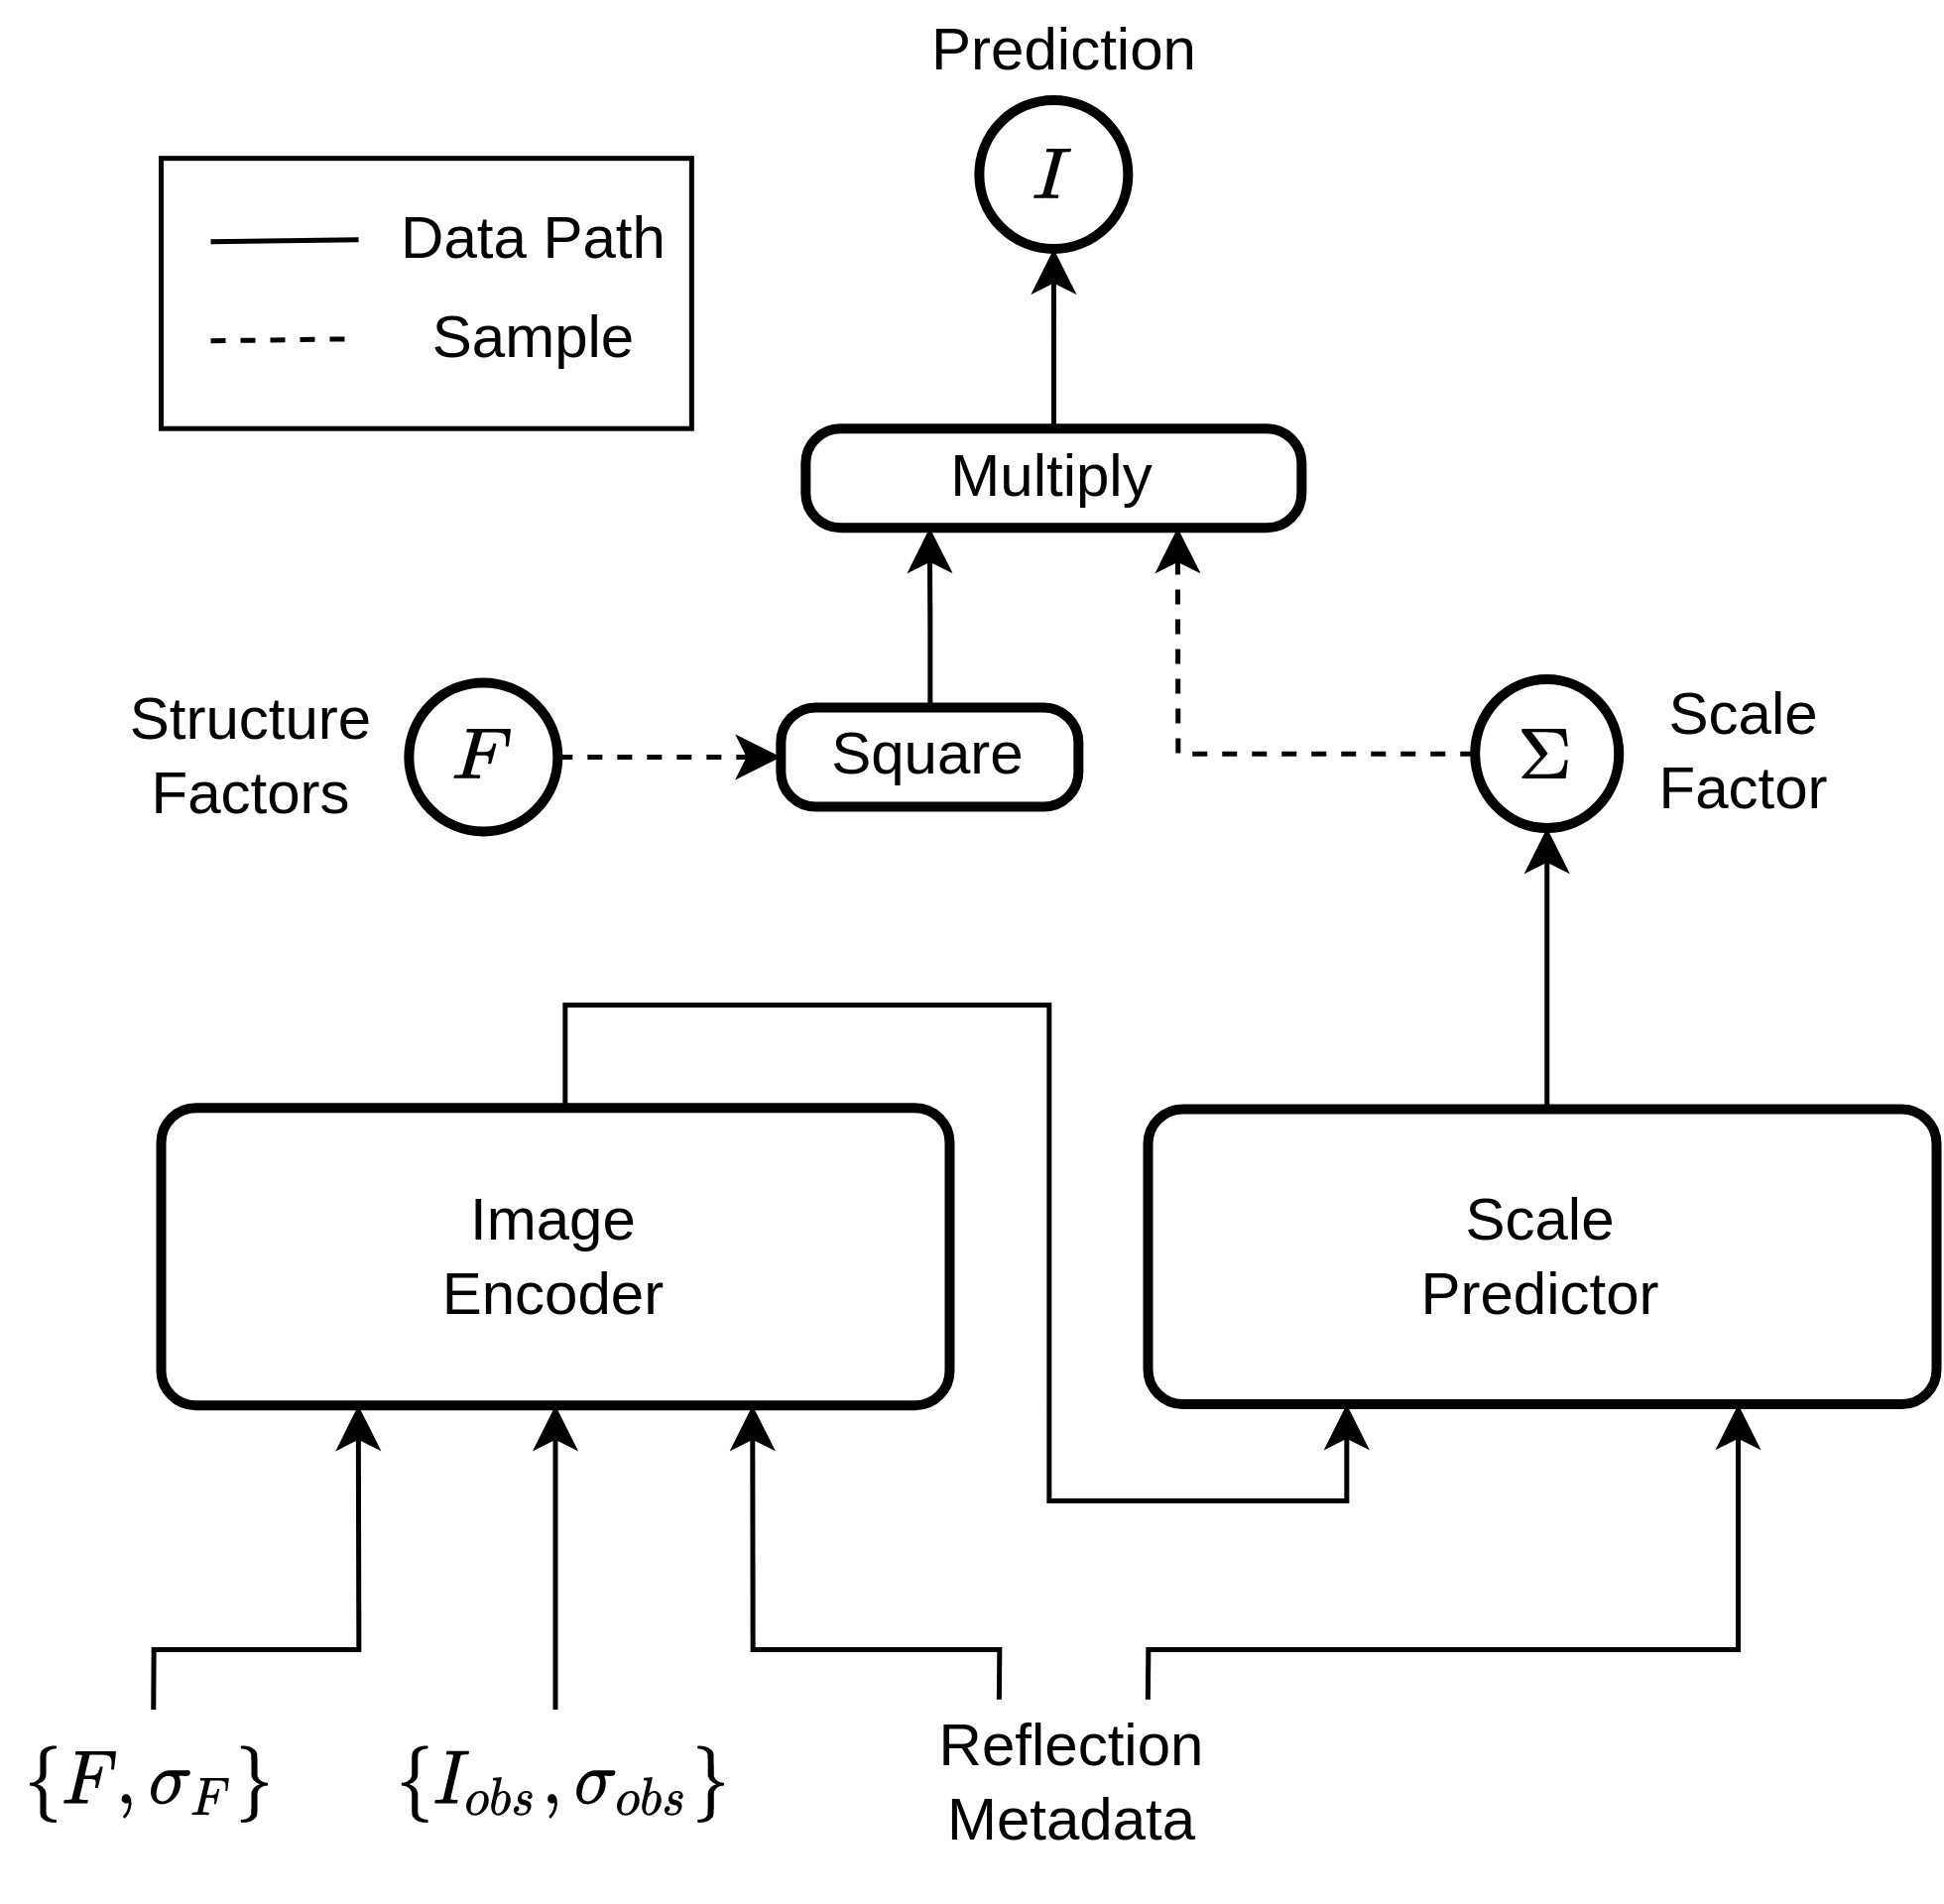
\includegraphics[width=\textwidth]{figures/model/overall.png}
        \end{figure}
    \end{minipage}

    In this model we choose to parameterize structure factors by a truncated normal distribution with positive support as in previous work \cite{dalton_careless_2021}. The optimization variables are indicated in bold. The scalar variable, $\mathbf{k}$, is a global scale parameter which is constrained to be positive. $\mathbf{k}$ is important to account for the the fact that the prior on $\Sigma$ has an arbitrary mean. $\mathbf{\mu_F}$ and $\mathbf{\sigma_F}$ are the location and scale parameters of the structure factor distributions. Both are constrained to be positive using the softplus function. We refer to the parameters of the scale model as $\mathbf{\theta}$. These consist exclusively of bias vectors and randomly initialized weight matrices in the linear layers of the model. In this implementation the first two terms of the $ELBO$ are estimated by drawing reparameterized samples \cite{kingma_auto-encoding_2014} from the structure factor distribution and scale distribution. The Kullback-Leibler divergence between the scales and their prior is computed analytically. The weight terms, $w_F$ and $w_\Sigma$, are hyperparameters which modulate the strength of the priors. During each training update, $\mathcal{L}$, is summed over the reflections in one image. 
  \end{alertblock}

  \begin{block}{Feed Forward Layer}
    \begin{figure}[t]
        \begin{subfigure}{0.3\textwidth}
            \centering
            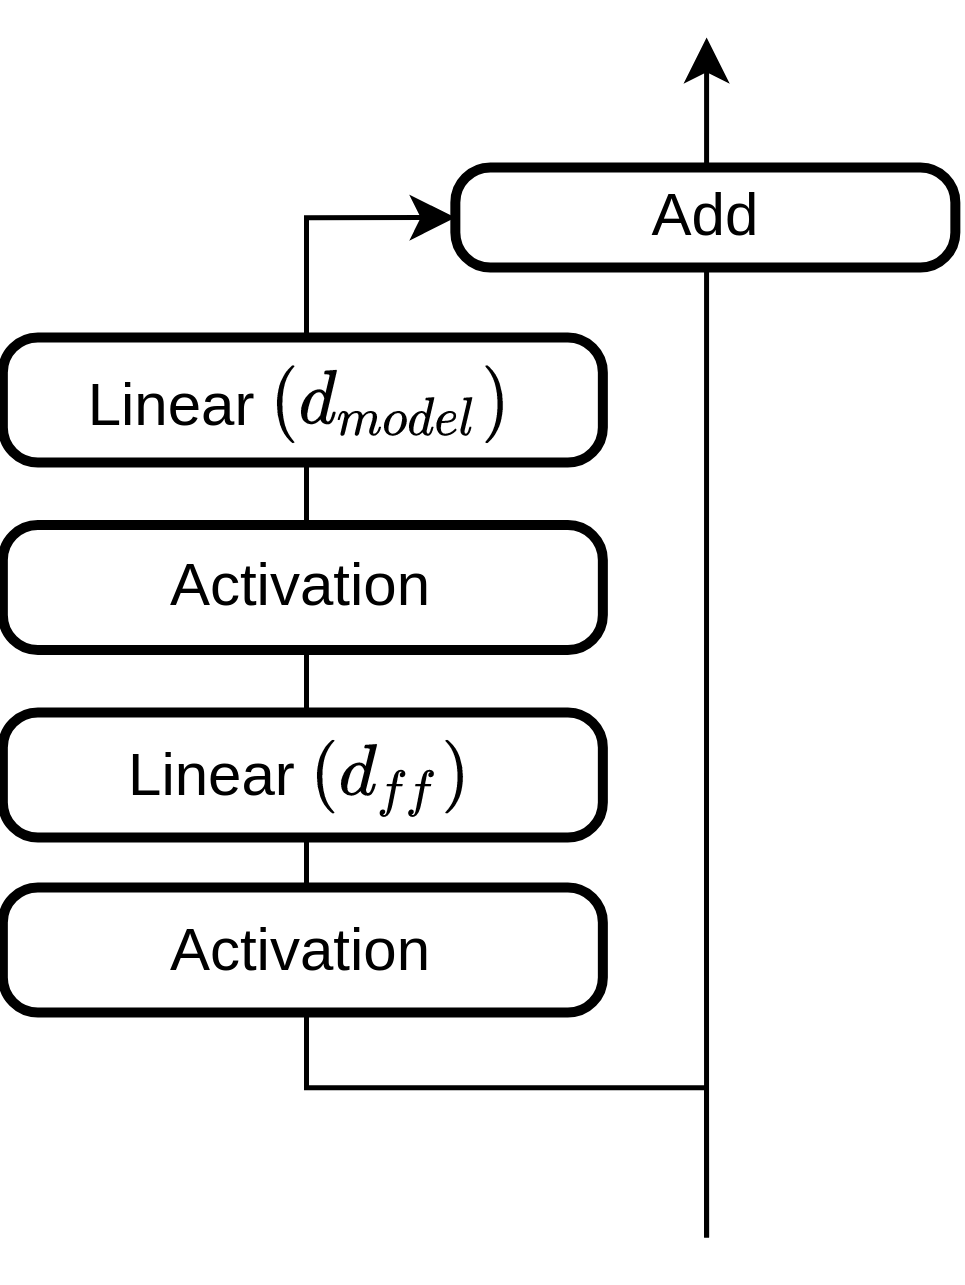
\includegraphics[width=0.80\textwidth]{figures/model/feedfoward.png}
        \end{subfigure}
        \begin{subfigure}{0.05\textwidth}
        \end{subfigure}
        \begin{subfigure}{0.6\textwidth}
            The fundamental nonlinear building block of the scale model is a \textbf{feed forward neural network}. This component of the model takes a batch of vectors with $d_{model}$ dimensions and outputs a modified batch of vectors in the same dimensional space. In this work, we use a ResNet version 2 block \cite{he_identity_2016}. The main advantage of this type of layer is that it contains a \textbf{residual connection} between the input and output. The output layer takes the elementwise sum of the input and a nonlinear projection thereof. This ensures that \textbf{gradients of the loss function do not vanish} in earlier layers leading to stalled learning. 
        \end{subfigure}
    \end{figure}
  \end{block}

\end{column}

\separatorcolumn

\begin{column}{\colwidth}

  \begin{block}{Image Encoder Model}
    \begin{figure}
        \begin{subfigure}[c]{0.45\textwidth}
            \centering
            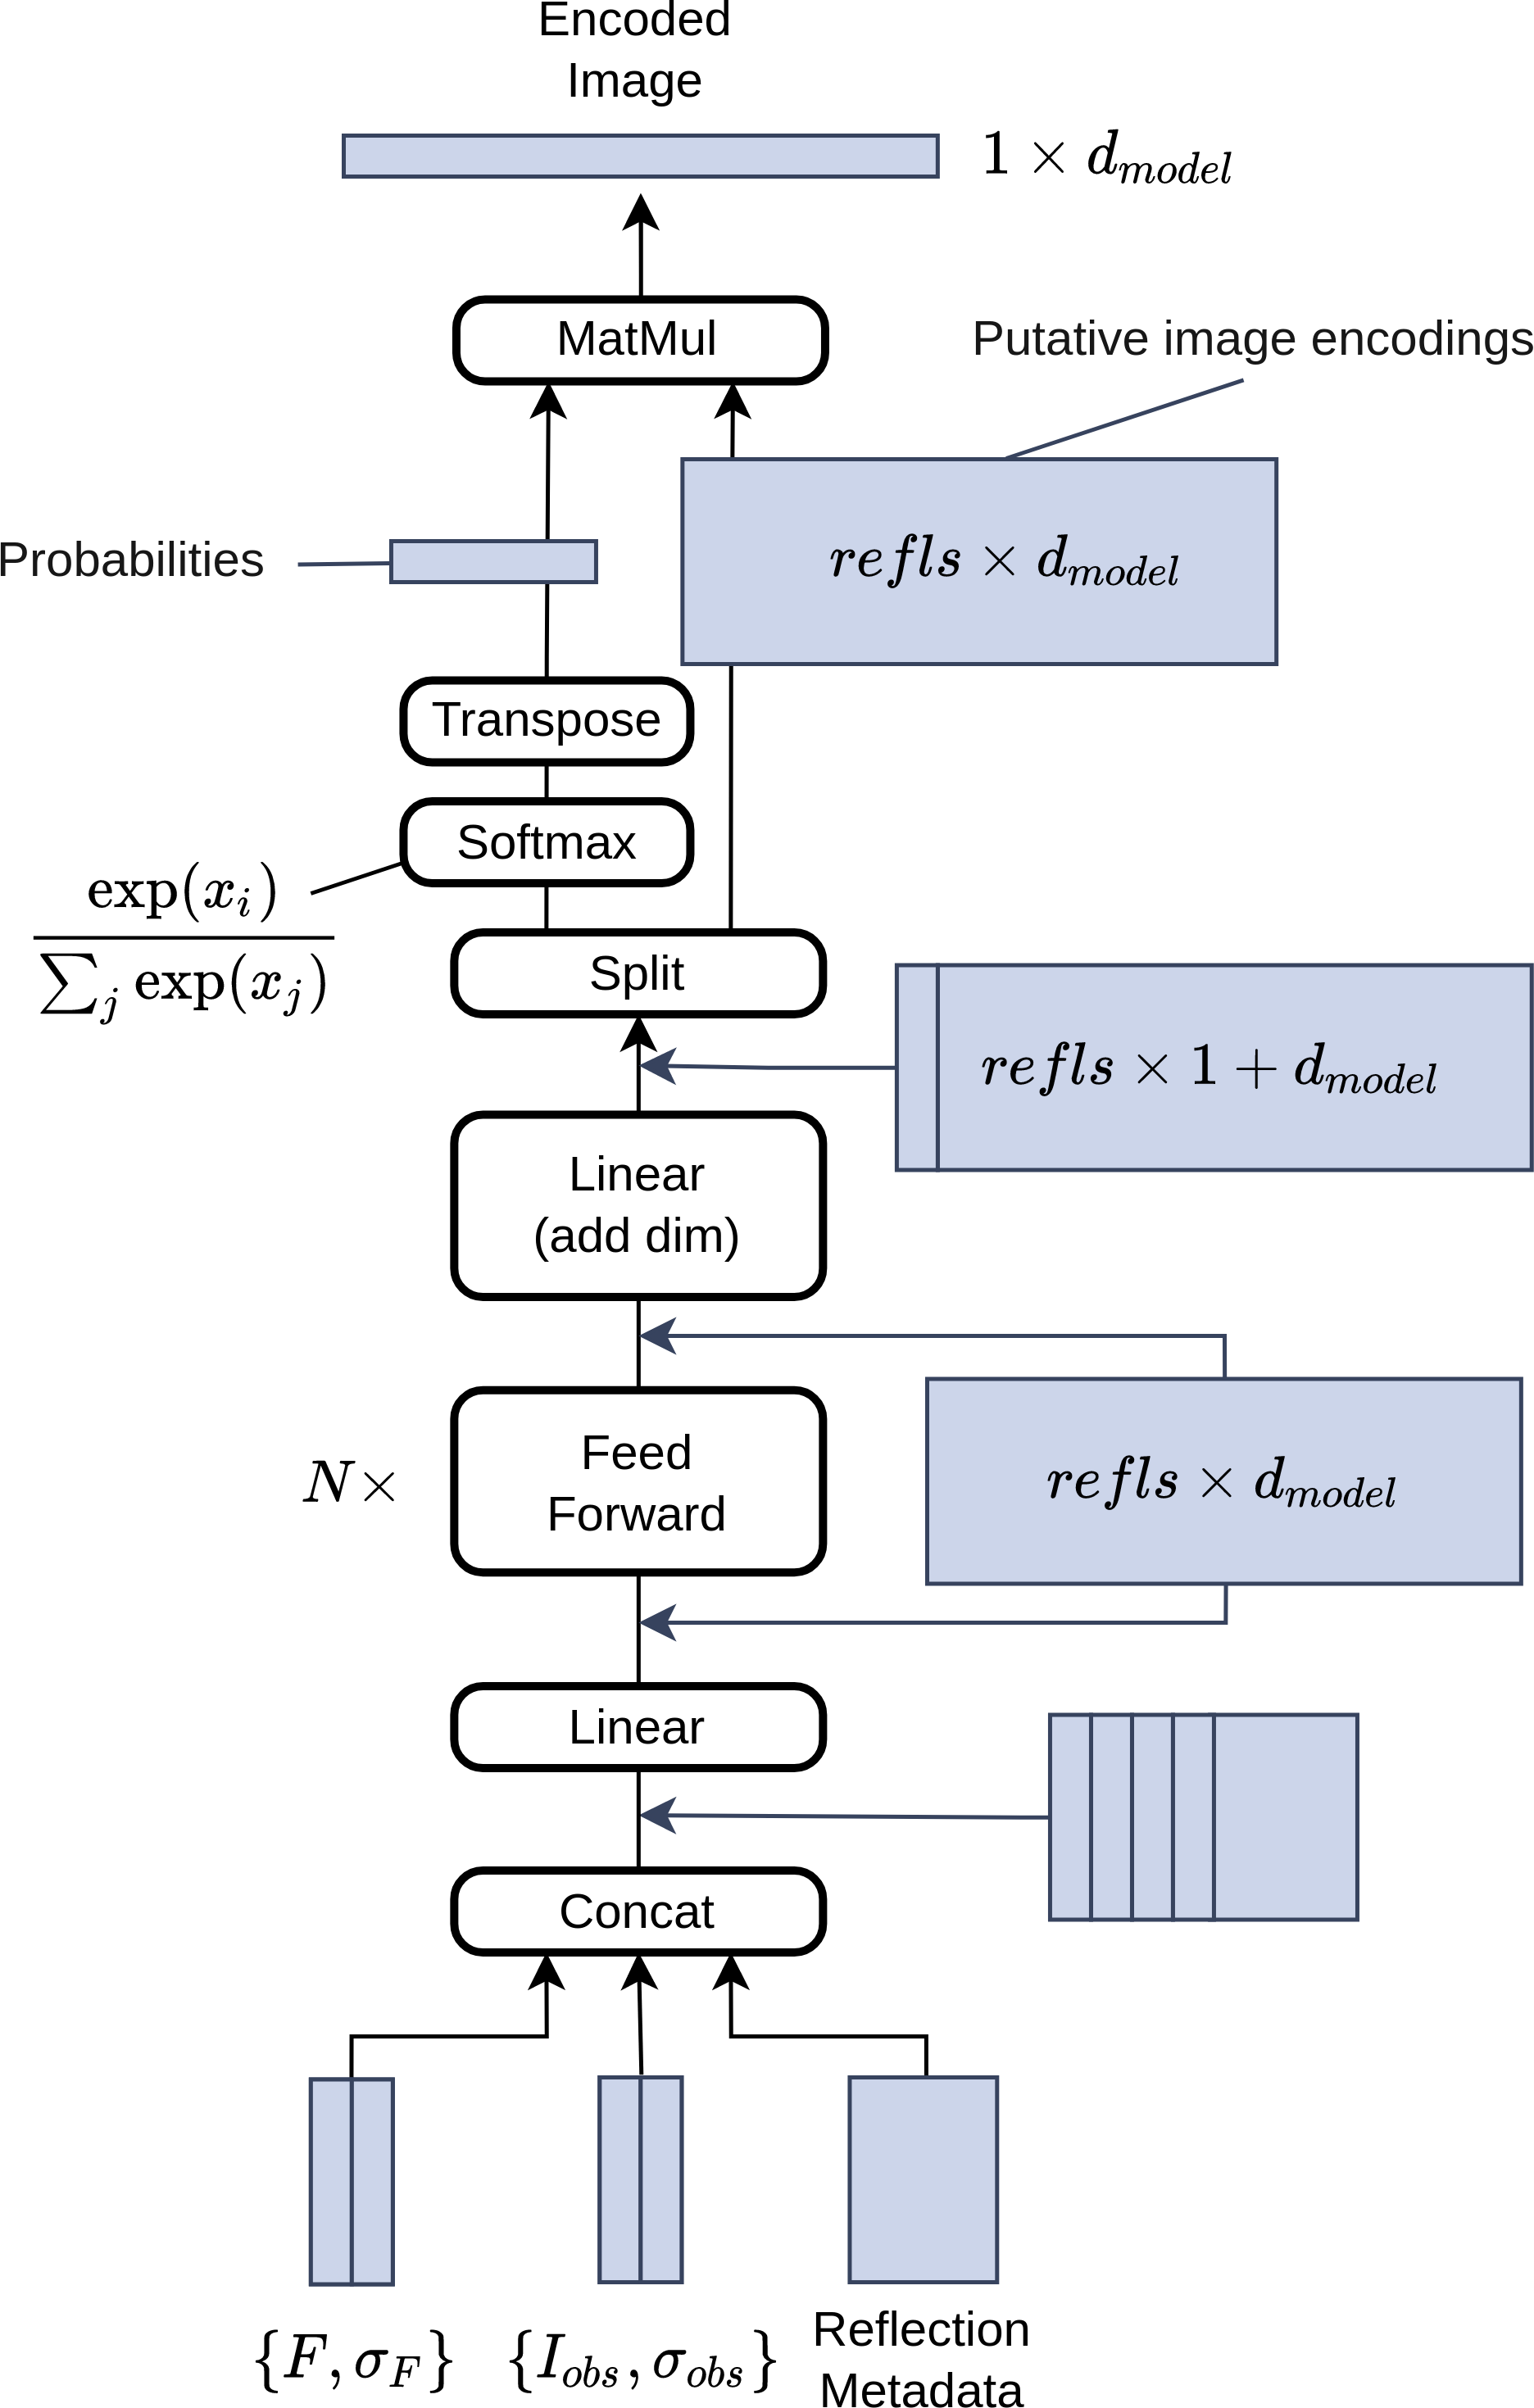
\includegraphics[width=0.9\textwidth]{
                %figures/model/image_encoder_harvardized_trimmed.png
                figures/model/image_encoder_mcbified_trimmed.png
            }
        \end{subfigure}
        \begin{subfigure}[c]{0.5\textwidth}
            The idea behind the image encoder is to learn a function which looks at the current structure factor estimates, the context of each reflection (reflection metadata), and the observed intensities and \textbf{suggests a vector that describes the image}. Hopefully, this vector includes information needed to scale the reflections on this image. For instance, the vector should encode information about the orientation of the crystal, its size, shape, and mosaic properties, the brightness and deflection of the X-ray beam, etc. The way this representation comes about is that a neural network \textbf{considers each reflection in isolation} and \textbf{proposes a putative image encoding} based on that reflection. Alongside the putative encoding, the network also \textbf{outputs a score} representing the probability that the reflection has something meaningful to say about the image overall. The consensus encoding is taken to be the sum over candidate encodings weighted by this probability. \textbf{Pooling the candidate encodings} into a single vector of length $d_{model}$ prevents this model from passing reflections' intensities directly to the scale model. This is \textbf{essential to prevent the overall model from overfitting} during training. 
        \end{subfigure}
    \end{figure}
  \end{block}
  \begin{block}{Reflection Scaling Model}
    \begin{figure}
        \begin{subfigure}[c]{0.5\textwidth}
           The goal of the scaling model is to produce a distribution of \textbf{probable scale factors} appropriate for each reflection in an image. As in previous work \cite{dalton_careless_2021}, it \textbf{uses metadata associated with each reflection} in order to infer scales. Unlike the previously published model, it has access to the \textbf{image representation produced by the upstream encoder model}. The input layers of this model simply concatenate the image vector onto each reflection's metadata. A neural network uses this enriched representation of the reflection to predict appropriate scale factors. In the parameterization presented here, the neural network predicts a two-vector interpreted as the location and scale parameters of a log-normal distribution. The LogNormal layer converts the scale parameter to a strictly positive number by applying the softplus function, $f(x) = \log(1 + exp(x))$.
        \end{subfigure}
        \begin{subfigure}[c]{0.45\textwidth}
            \centering
            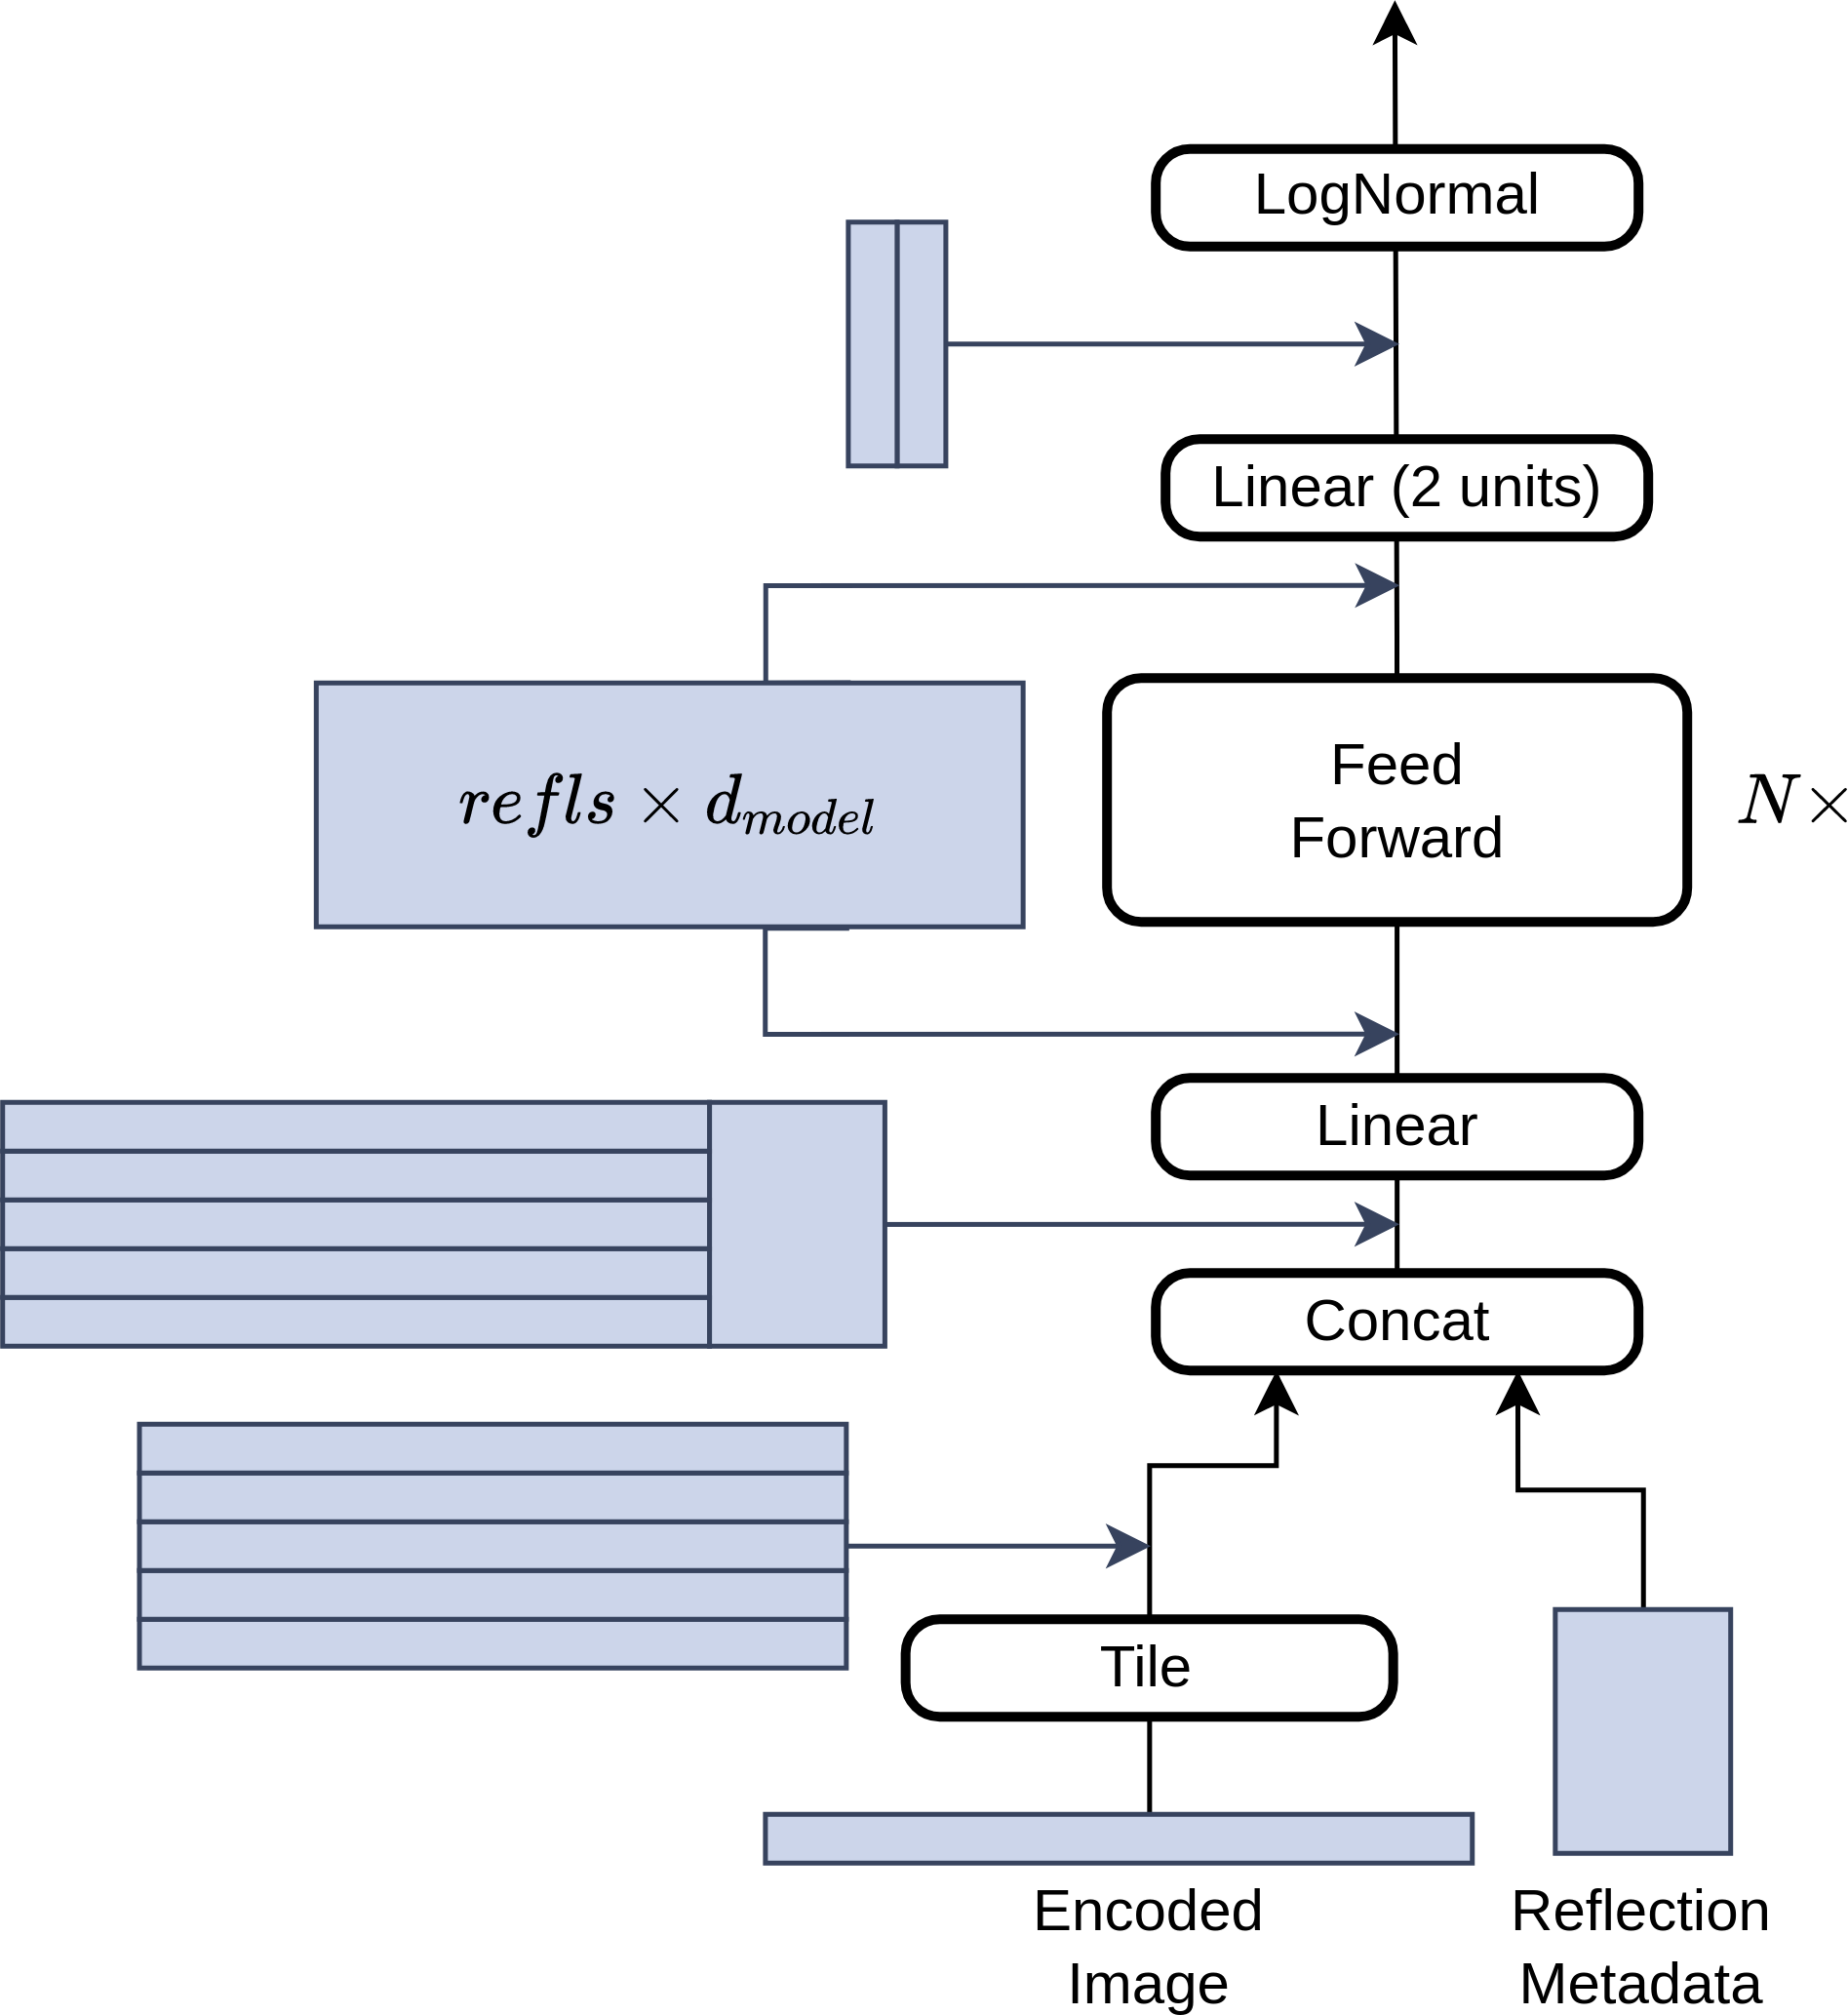
\includegraphics[width=0.9\textwidth]{
                %figures/model/scale_harvardized_trimmed.png
                figures/model/scale_mcbified_trimmed.png
            }
        \end{subfigure}
    \end{figure}
    
  \end{block}
  \begin{block}{Example Application to Single Wavelength Anomalous Diffraction Data}
  As a case study for the suitability of this model for merging \textbf{serial femtosecond crystallography} data, we applied it to a publicly available dataset consisting of \textbf{166,250 diffraction images} \cite{kern_taking_2014} of the \textbf{zinc metalloprotease, thermolysin}, which were integrated using DIALS \cite{brewster_improving_2018} (CXIDB: 81). The data were acquired at a wavelength of 1.27 Å leading to considerable anomalous signal from the zinc ions in the active site. In addition to zinc, thermolysin also has four ordered calcium ions and two methionine residues which may contribute anomalous signal. We trained our model for \textbf{500,000 gradient updates} using the Adam optimizer for stochastic objective functions \cite{kingma_adam_2017}. This equates to slightly more than \textbf{3 passes over the dataset}. We trained the model on a consumer GPU (NVIDIA RTX 3060). With the reported hyperparameters, the model requires \textbf{797 megabytes} of GPU memory and executes a gradient step in roughly 70ms. Total training time was \textbf{less than 12 hours}. By optimizing the input pipeline and tuning hyperparameters, we expect a 3 to 10-fold speedup is attainable. 

  \begin{figure}[]
    \centering
    \begin{subfigure}[c]{0.60\textwidth}
      \centering
      Training trajectory\bigskip
      
      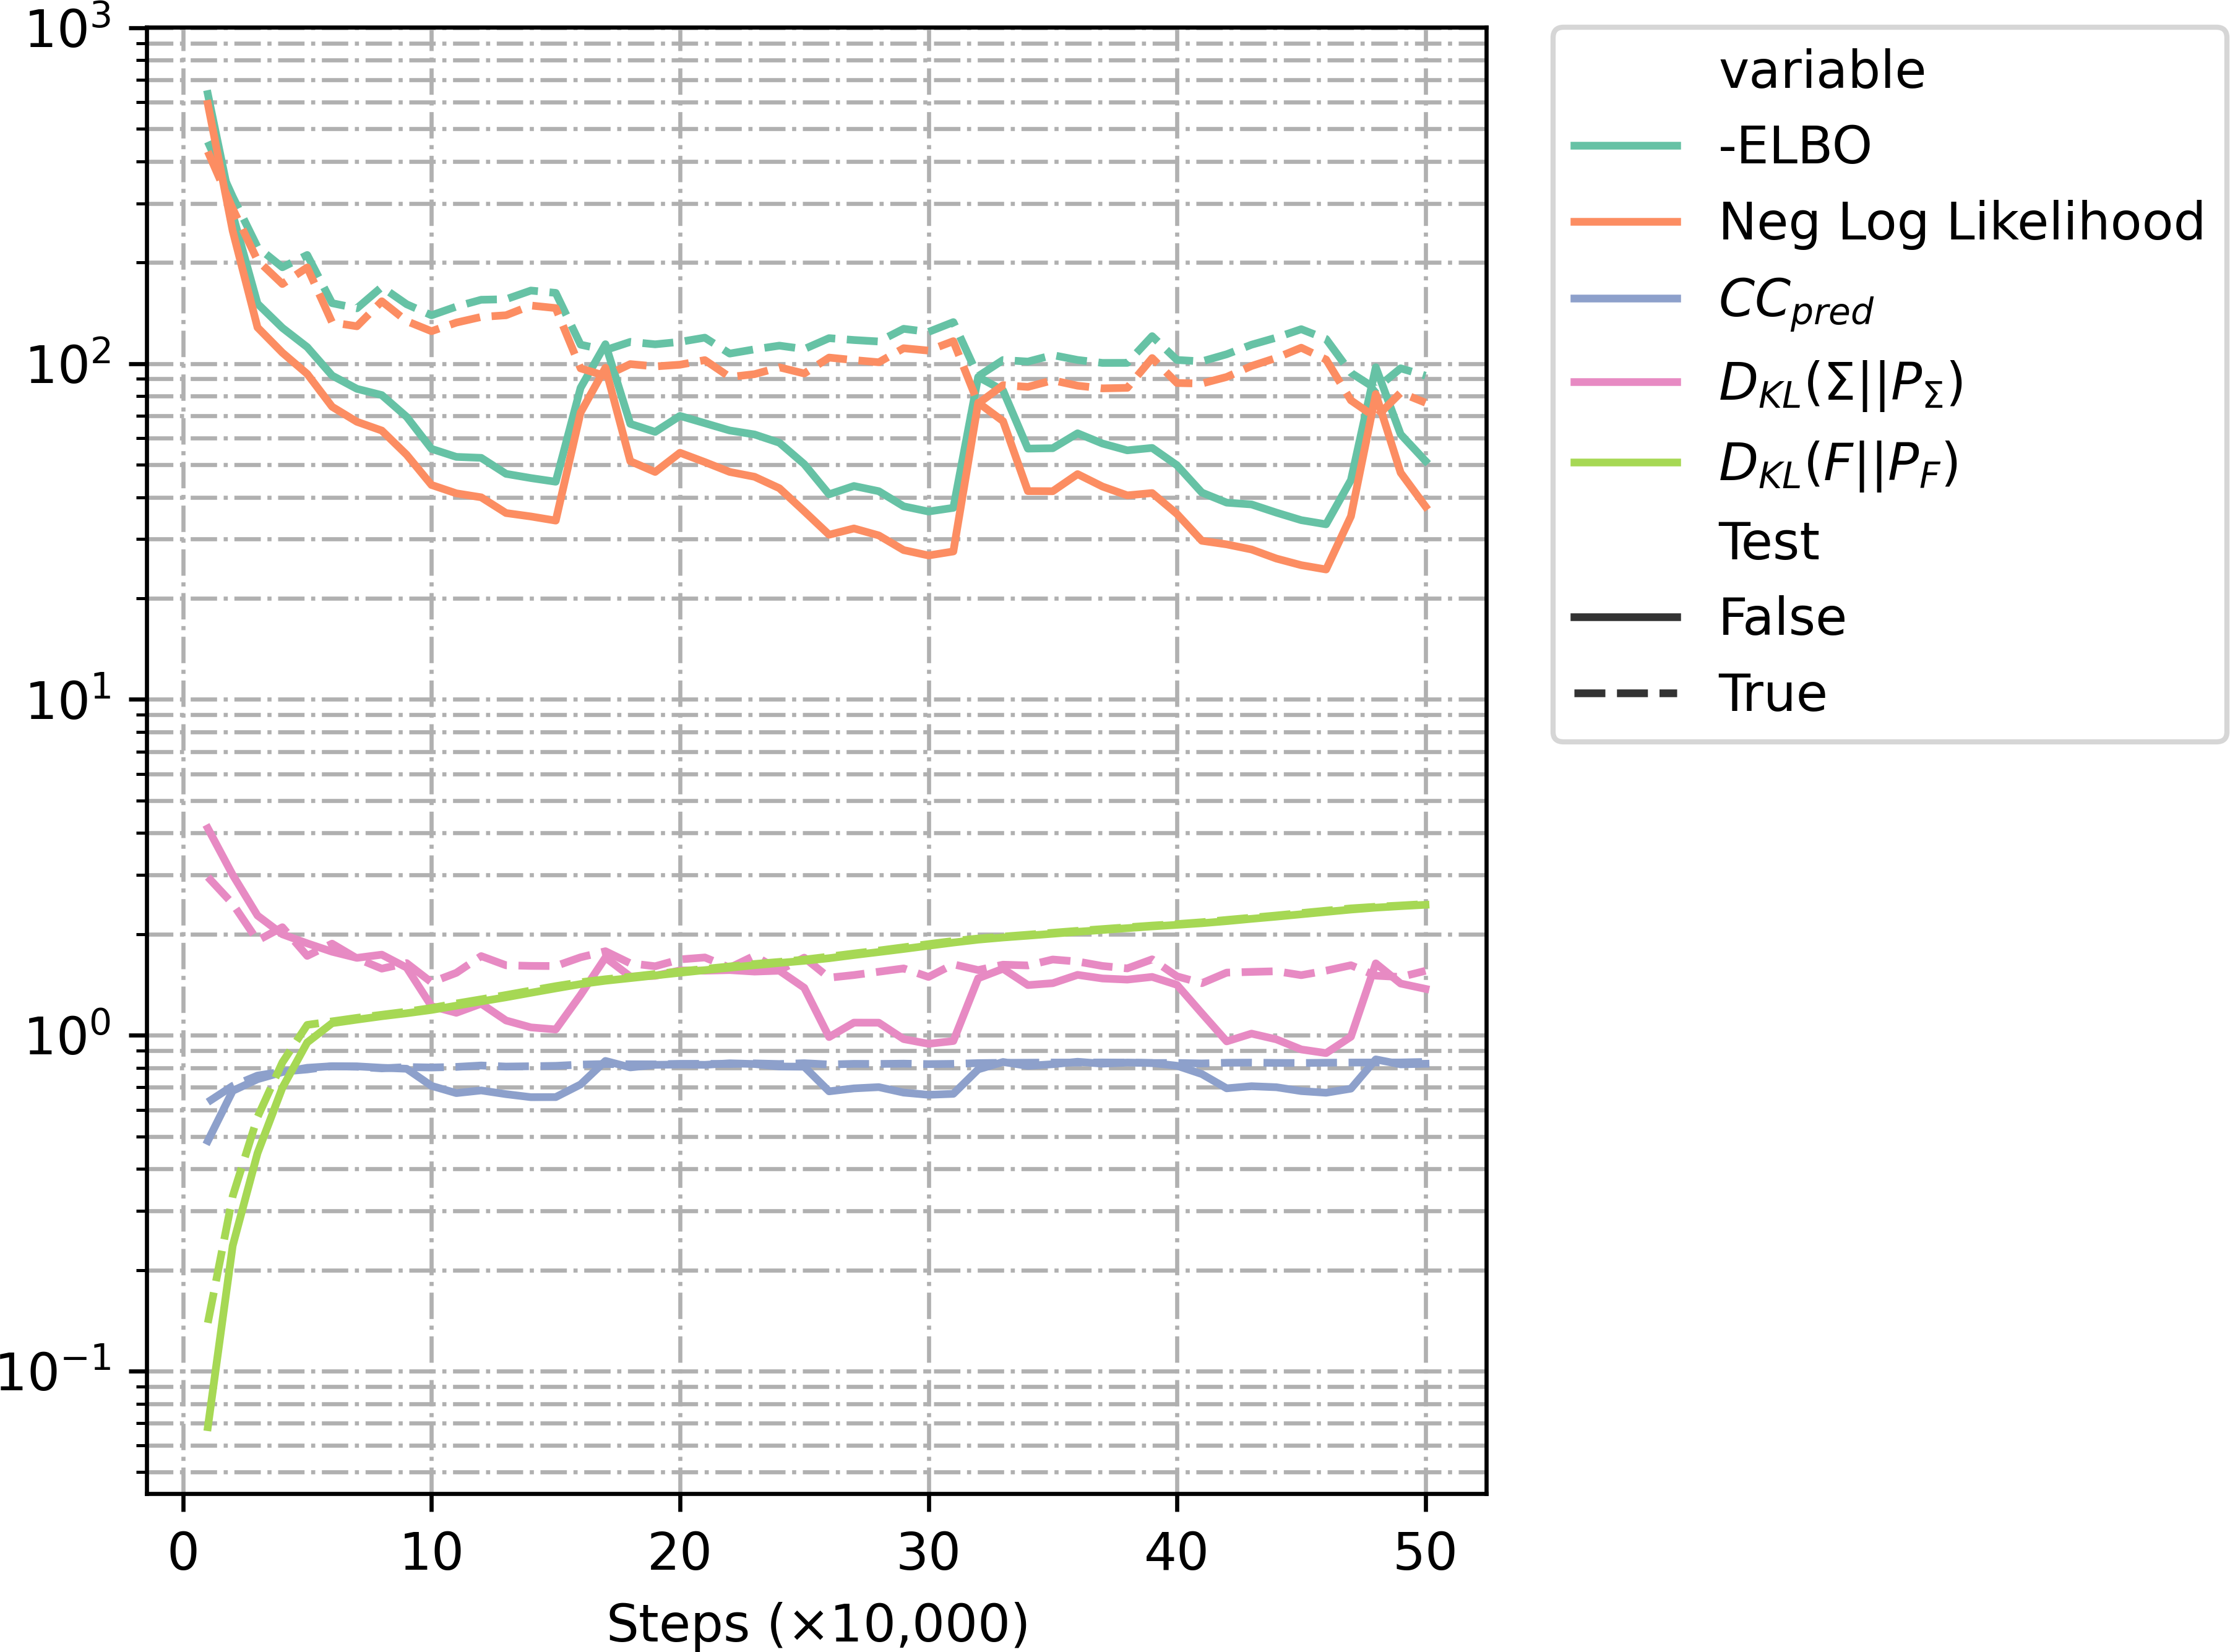
\includegraphics[width=\textwidth]{figures/thermolysin/trajectory_trimmed.png}
    \end{subfigure}\hfill
    \begin{subfigure}[c]{0.35\textwidth}
      \centering
      Model hyperparameters\bigskip

      \begin{tabular}{c|c}
           \hline 
           Metadata & Scattered wavevector, \\
                    & Ewald offset vector (Å\textsuperscript{-1}) \\
           Activation & $ReLU$ \\
           $N$ & 20\\
           $d_{model}$ & 32\\
           $d_{ff}$ & 64\\
           $w_{F}$ & $0.001$ \\
           $w_{\Sigma}$ & $10$ \\
           $S$ (samples) & 50 \\
           Learning rate & 0.001 $\times 50k$ \\ 
           & 0.0001 after\\
           $\beta_1$ & 0.9 \\
           $\beta_2$ & 0.999 \\
      \label{tab:hyperparameters}
      \end{tabular}
    \end{subfigure}
      %\begin{tabular}{c c}
      %     $S_1x$ & x-coordinate of the scattered beam wave vector \\
      %     $S_1y$ & y-coordinate of the scattered beam wave vector \\
      %     $Q_{x} - Q_{obsx}$ & x-coordinate of Ewald offset vector \\
      %     $Q_{y} - Q_{obsy}$ & y-coordinate of Ewald offset vector \\
      %     $Q_{z} - Q_{obsz}$ & z-coordinate of Ewald offset vector \\
      %\end{tabular}
      %\caption{Metadata for merging serial crystallography data}
      %\label{tab:metadata}
  \end{figure}
  \end{block}

\end{column}

\separatorcolumn

\begin{column}{\colwidth}
  
  \begin{block}{Thermolysin Phasing Results}
  \begin{figure}[]
    \begin{subfigure}[t]{0.5\textwidth}
      \centering
      Anomalous signal during training\bigskip

      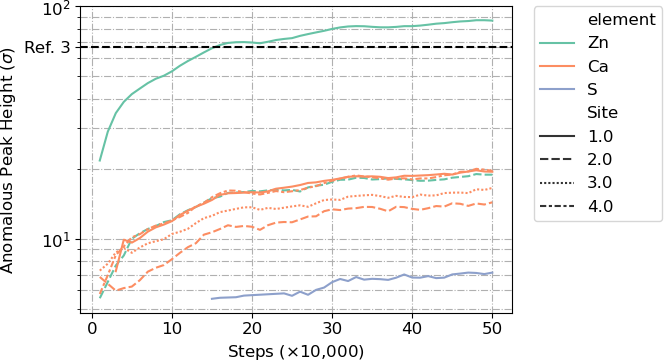
\includegraphics[width=\textwidth]{figures/thermolysin/anom_peaks_annotated_trimmed.png}
    \end{subfigure}\hfill
    \begin{subfigure}[t]{0.45\textwidth}
      \centering
      Comparison of SAD phasing results \bigskip

      \bgroup
      \def\arraystretch{1.5}%  1 is the default, change whatever you need
      \begin{tabular}{r|c|c}
            & Ours & Reference \cite{brewster_sad_2019} \\
            \hline
            Zn\textsuperscript{2+} peak ($\sigma$) & 83.2 & 67.0 \\
            Model-map CC & 0.84 & 0.80$\pm$0.001 \\
            Sites found & 7 & 6 \\
            Residues built & 305 & 297.2$\pm$6.5 \\
            $R_{work}$ & 0.204 & 0.212$\pm$1.3 \\
            $R_{free}$ & 0.231 & 0.237$\pm$1.7 \\
      \end{tabular}
      \egroup
      \label{tab:phasing}
    \end{subfigure}
      \RaggedRight
      \bigskip
        
      The table presents SAD Phasing Results from AutoSol \cite{terwilliger_decision-making_2009} using the same parameters as \cite{brewster_sad_2019}. The zinc peak height in the table is from \texttt{phenix.find\_peaks\_holes} using our structure factor estimates and the autobuilt model. 
  \end{figure}
  
  \begin{figure}[]
    \begin{subfigure}[t]{0.45\textwidth}
      \centering
      Thermolysin active site\bigskip

      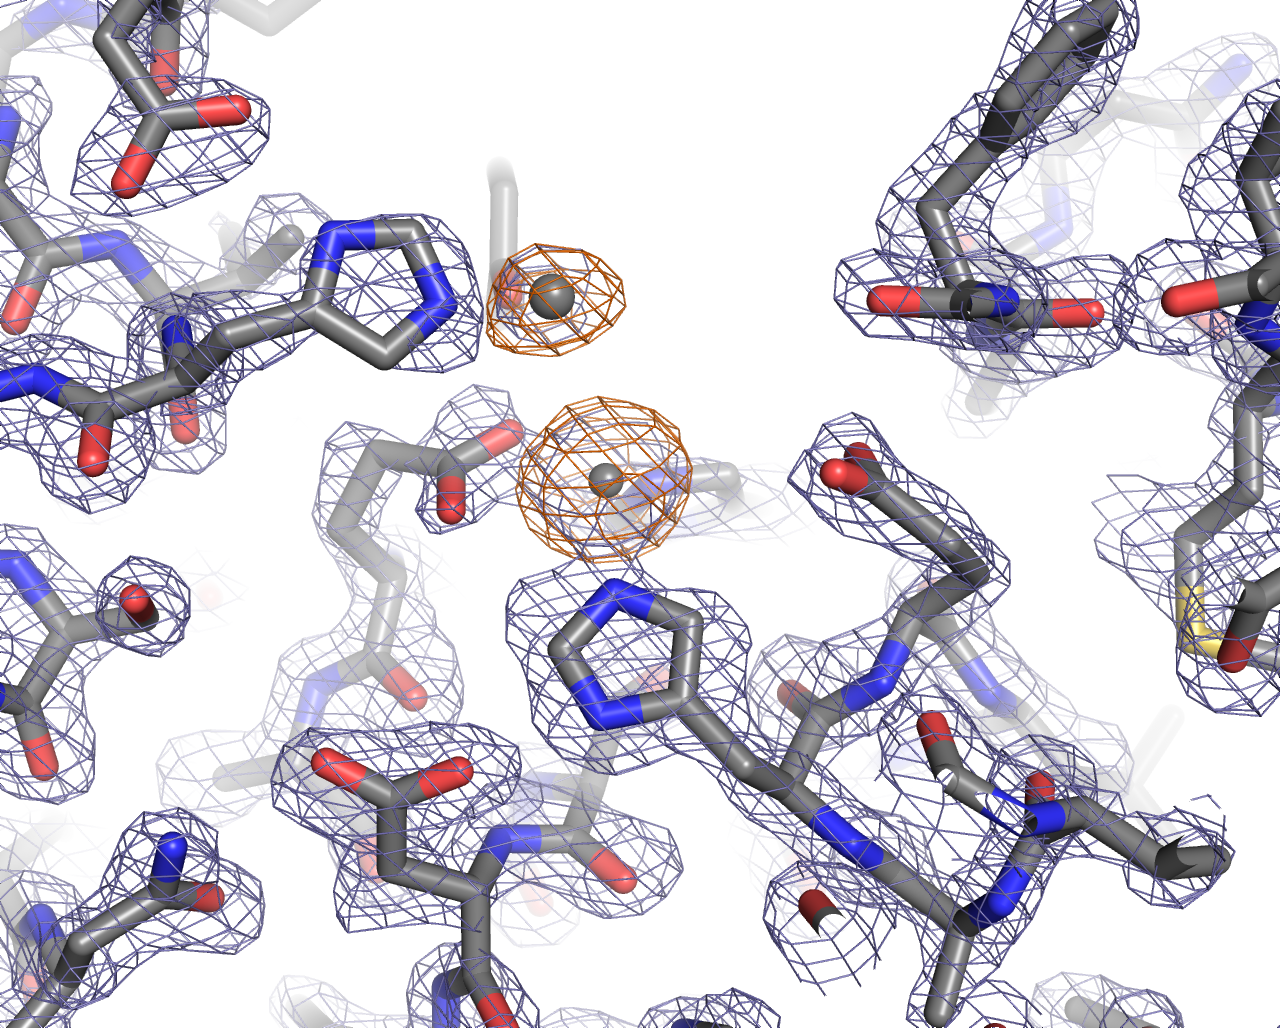
\includegraphics[width=\textwidth]{figures/thermolysin/zinc.png}
    \end{subfigure}\hfill
    \begin{subfigure}[t]{0.45\textwidth}
      \centering
      Methionine-205\bigskip

      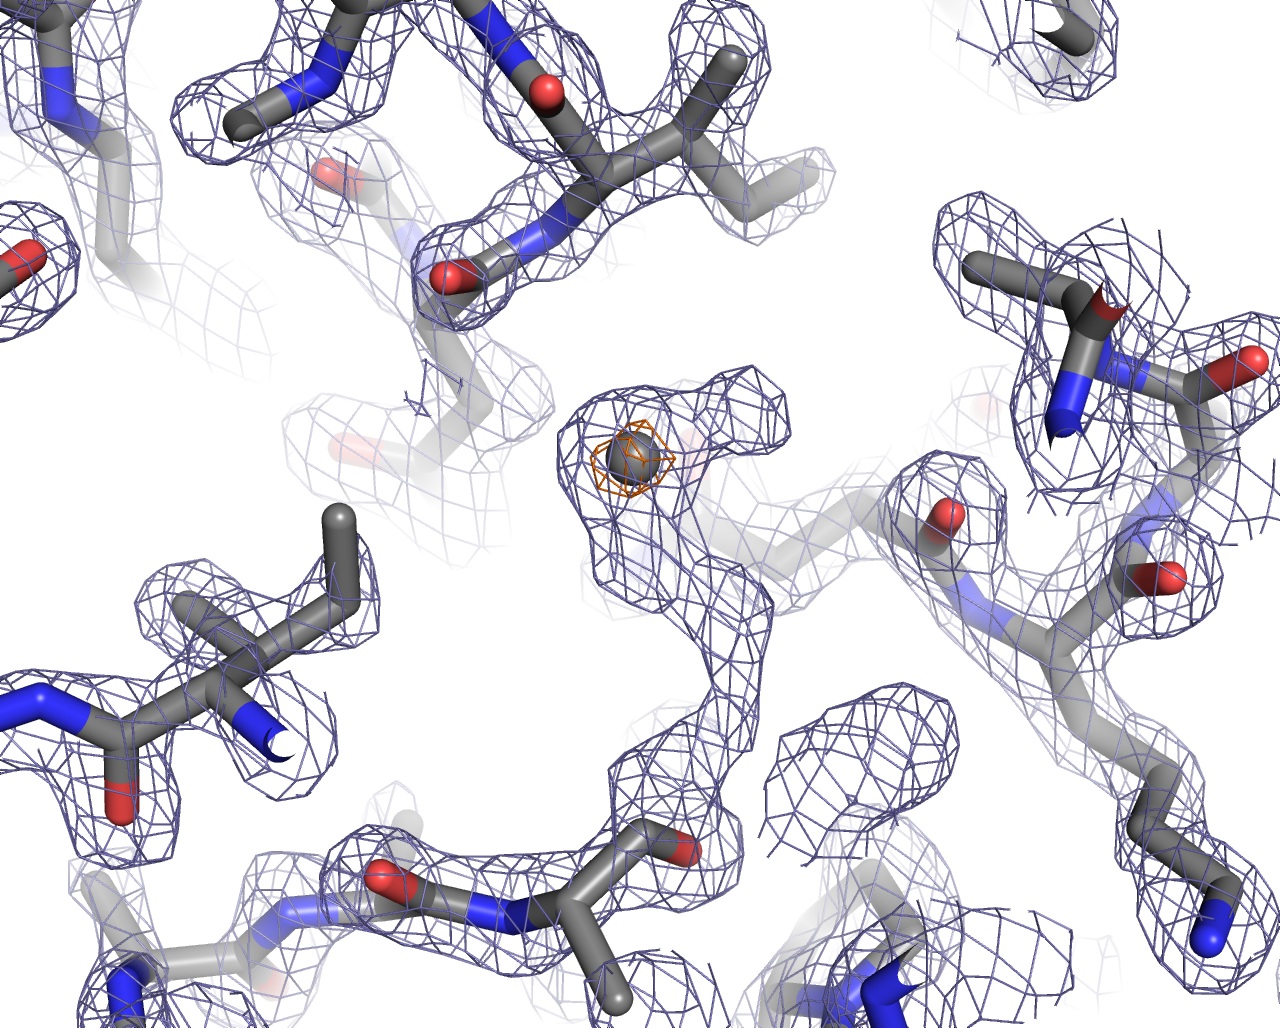
\includegraphics[width=\textwidth]{figures/thermolysin/sulfur_2.png}
    \end{subfigure}
    \RaggedRight
    \bigskip

    Thermolysin SAD phasing results featuring the \textbf{autobuilt model from AutoSol} \cite{terwilliger_decision-making_2009}. The blue electron density, contoured at 2$\sigma$, is the \textbf{experimental, density-modified map}. The orange map is the \textbf{anomalous difference map} using the pictured model for phases and the structure factor estimates from our merging algorithm contoured at 5$\sigma$.
  \end{figure}
  
  \end{block}
  


%Presently, the performance is limited by i/o overhead. If the data can be cached in system memory, the model trains approximately $3\times$ faster. We expect to obtain such performance for datasets too large to fit in memory by optimizing the input pipeline. right now the FOM on this

  \begin{block}{Acknowledgements}
  We would like to thank Aaron Brewster, Derek Mendez, and Jack Greisman for many helpful conversations about crystallography. 
  We are grateful to Minhuan Li and John Russell for input on machine learning algorithms and libraries. 
  This work was supported by the Searle Scholarship Program (SSP-2018-3240), a fellowship from the George W. Merck Fund of the New York Community Trust (338034), and the NIH Director's New Innovator Award (DP2-GM141000).
  KD holds a Career Award at the Scientific Interface from the Burroughs Wellcome Fund. 
  
  \end{block}
  
  \begin{block}{References}

  \printbibliography
  %\nocite{*}
  %\footnotesize{\bibliographystyle{unsrtnat}\bibliography{poster}}

  \end{block}

\end{column}

\separatorcolumn
\end{columns}
\end{frame}

\end{document}
